\begin{frame}
  \begin{center}
    \LARGE <<Подарок>>
  \end{center}

  \begin{center}
      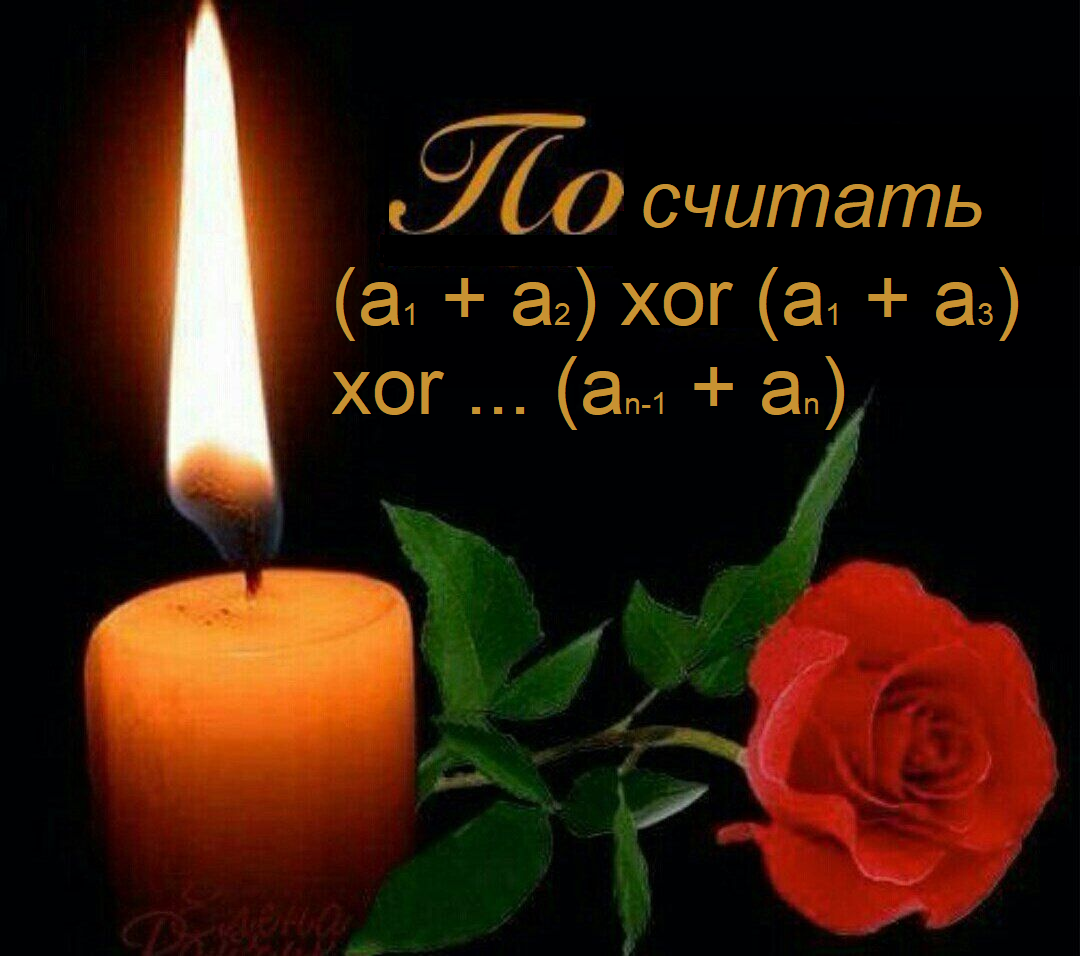
\includegraphics[width=5cm]{memes/e-meme.png}
  \end{center}

  \begin{itemize}
  \item Идея задачи --- Грикукан
  \item Разработка задачи --- Александр Курилкин
  \end{itemize}

\end{frame}

\begin{frame}{Постановка задачи}

  \begin{itemize}
  \item Дан массив чисел, нужно посчитать побитовый xor сумм всех пар чисел в нем
  \end{itemize}

\end{frame}

\begin{frame}{Решение за $\O(n^2)$ (15 баллов)}
  \begin{itemize}
  \item Двойным for явно переберем все пары и посчитаем ответ.
  \end{itemize}
\end{frame}

\begin{frame}{Решение за $\O(n + C^2)$ (20 баллов)}
  \begin{itemize}
  \item Посчитаем количество каждого числа;
  \item После этого двойным for переберем все возможные пары значений чисел;
  \item Пусть значения равны $i$ и $j$;
  \item Если $i \neq j$, то если $cnt_i \cdot cnt_j \bmod 2 = 1$, то $i + j$ войдет в считаемое выражение нечетное кол-во раз, и его нужно учесть (проксорить $ans$ с $i + j$), иначе нет;
  \item Если $i = j$, то делаем все то же, только теперь кол-во раз, которое $i + i$ войдет в выражение, считается по формуле $\frac{cnt_i \cdot (cnt_{i} - 1)}{2}$.
  \end{itemize}
\end{frame}

\begin{frame}{Полное решение}
  \begin{itemize}
      \item Будем считать каждый бит в ответе отдельно. Пусть мы хотим посчитать, чему равен $k$-й (в 0-индексации) бит;
      \item Заметим, что тогда от чисел нас интересуют только их биты от $0$-го до $k$-го, то есть можно взять все числа по модулю $2^{k + 1}$;
      \item Теперь сумма двух чисел может не превышать $2^{k + 2} - 2$, при этом $k$-й бит равен 1, если эта сумма попадает в отрезок от $[2^k; 2^{k + 1})$ или $[2^{k + 1} + 2^k; 2^{k + 2} - 2]$.
  \end{itemize}
\end{frame}

\begin{frame}{Полное решение}
  \begin{itemize}
      \item Осталось посчитать кол-во пар чисел, дающих такую сумму. Для этого отсортируем все взятые по модулю $2^k$ числа и пройдемся двумя указателями или сделаем бинпоиски для каждого числа;
      \item Итоговое время работы: $O(n \log n \log C)$;
      \item Бонус: можете убрать $\log n$ из асимптотики?
  \end{itemize}
\end{frame}
